\section{Bladder Cancer}


% Overview of the bladder cancer stats
According to Cancer Research UK, bladder cancer is the 10th most common cause of cancer and the 11th most common cancer in the UK \cite{Cancer_Research_UK2015-cf}. This is equivalent to ~10,000 cases from which  ~5000 are deaths, with a 5-year survival rate of 52.6\%. Patients diagnosed with bladder cancer undergo periodical cystoscopies and in the case of the muscle invasive, the patient may suffer from cystectomy which removes the entire bladder. This leads to a poor quality of life of the patients but also to high costs to the healthcare systems. 

% The two types of bladder 

\begin{figure}[!htb]    
    \centering
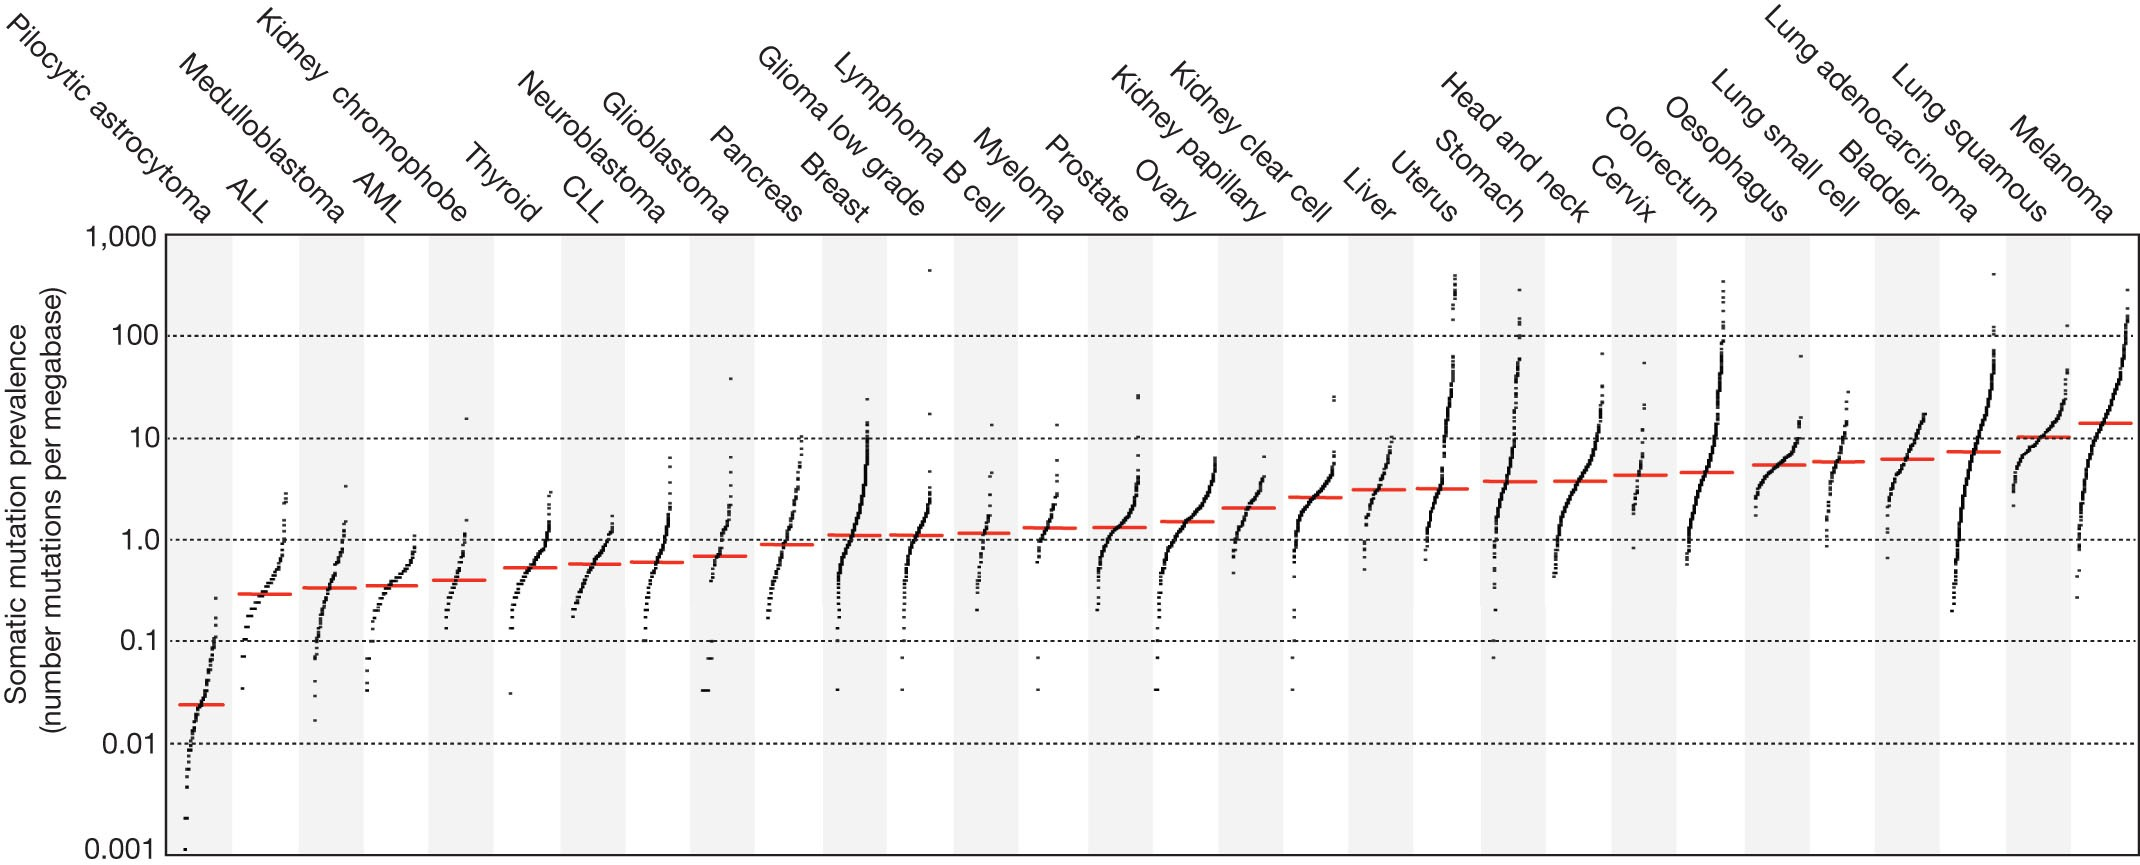
\includegraphics[width=0.9\textwidth,height=0.9\textheight,keepaspectratio]{Sections/Lit_review/Resources/mut_sig_cancers.jpg}
    \caption{Image from \cite{Alexandrov2013-gi} showing the somatic mutations across the different human cancer. Each sample is represented by a dot and the red line is the median number of mutation in that tumour type. The y-axis is the number of mutations per megabases, and the cancer types are ordered by the median mutation count, which makes bladder cancer the 4th highest mutated cancer.}
    \label{fig:lit:cancer_mut_sig}
\end{figure}

% Some properties of the bladder cancer
% - highly mutated, a lot of epginetic changes
The research conducted by \citet{Alexandrov2013-gi} studies the mutational signatures across the human tumour types, covering ~7000 cancer samples from which 20 distinct mutational signatures were extracted. \Cref{fig:lit:cancer_mut_sig} shows the mutation burden across the tumour types, with the skin cancer being the most mutated type. The bladder cancer has the 4th highest mutation burden with Signatures 13, 2 and 5 from COSMIC database\cite{Tate2019-yj}. Signature 2 and 13 are related to APOBEC family activity which are triggered by immune response. Signature 5 is unknown but it is thought to related to the mutations accumulated through ageing. 

\begin{figure}[!htb]    
    \centering
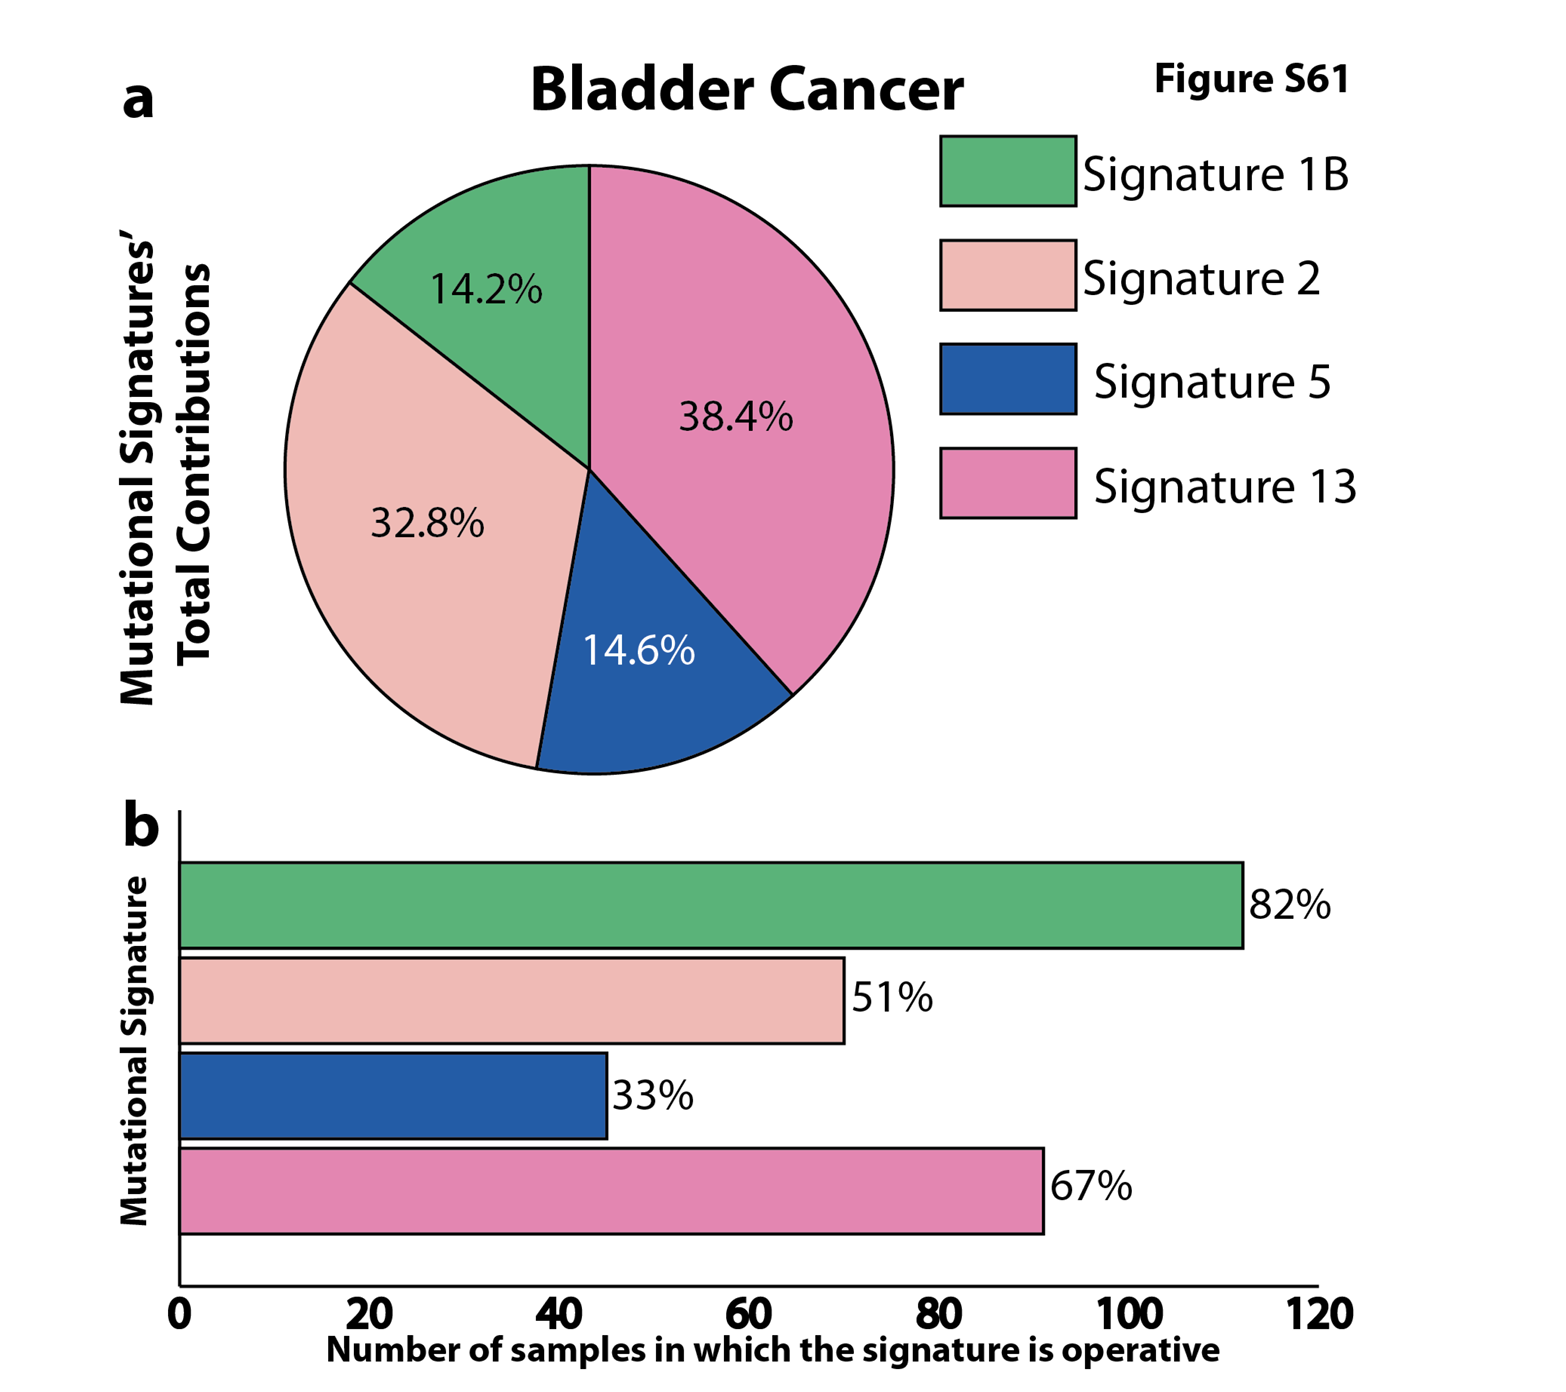
\includegraphics[width=0.6\textwidth,height=0.6\textheight,keepaspectratio]{Sections/Lit_review/Resources/bladder_mut_sig.png}
    \caption{Image from Supplementary \cite{Alexandrov2013-gi} showing the mutation signatures for bladder cancer. a) showing the the contribution of each signature while b) the number of samples where it was found. }
    \label{fig:lit:bladder_mut_sig}
\end{figure}


% epigenetic burden
The high somatic mutation burden is also highlighted by other research \cite{Cancer_Genome_Atlas_Research_Network2014-hb, Robertson2017-mg, Kamoun2020-tj}. The first two studies found that the mutations disrupt the epigenetic machinery. Understanding these anomalies have the potential to lead to new potential targeted treatments.

% Introduction of TCGA
There are two comprehensive studies of the muscle-invasive bladder cancer (MIBC) cohort from The Cancer Genome Atlas (TCGA) \citet{Cancer_Genome_Atlas_Research_Network2014-hb} and \citet{Robertson2017-mg}. The first is the initial research analysing the fist batch of patient samples (131) while the other analysed the entire cohort of 412 patient samples. The MIBC cohort from TCGA is an invaluable asset for the research community as a number of sequencing techniques were applied to the samples: mRNAseq (gene expression), WEX and WGS (somatic mutations), microarray-based (copy number variations) as well as metadata about the patients. This cohort is characterised by aggressive tumours, having a high grade muscle invasive.

% Talk about the TCGA subtypes
In the work of \citet{Robertson2017-mg} the multi-omics data is analysed separately, centering on the subgroups derived from gene expression and then correlating with the other data analysis. The main result being the stratification of the MIBC into five distinct molecular subtypes: $35\%$- Luminal Papillary (LumP), $19\%$ Luminal infiltrated (LumInf), $6\%$ Luminal, $35\%$ Basal Squamous (Ba/Sq) and $5\%$ Neuronal. The highest 5-year survival is given by the Luminal subgroups while the Neuronal has the worst prognosis. 

% Introducing the consensus work

\begin{todolist}
    \item Overview of the bladder cancer 
    \begin{todolist}
        \item [\done] Statistics worlwide/UK/Europe
        \item Main causes, metal contamination
        \item More prevalent in men
    \end{todolist}
    \item Why it is so bad? 
    \begin{todolist}
        \item [\done] Impact of the quality of life, treatment cost?
        \item Metastasis sites
    \end{todolist}
    \item Efforts to solve it and introduce the subtypes problem
    \item Introduce the consensus, TCGA and Lund
    \item Talk about the current UK trial that is using TCGA subtypes, stressing the importance of finding the right subgroups

\end{todolist}

\subsection{Tissue types of bladder cancer?}

\subsubsection{TCGA}


% Cover the Data in TCGA

% RNA-seq data

% Mutations

% Copy Number variation

% What type of tissue samples were used, more aggresive tumours

% How long did the study lasted, some of the relevant publications

\subsubsection{Consensus}

\subsubsection{Lund}

% How did they combined the different datasets


\subsection{Non-cancerous dataset}

% What are the three different types of tissues used?

% From which datasets where those used? Bladder vs Uropathies

% Properties of P0, Abs-Ca and Undifferentiated. Why it is important to include all of this? Abs-Ca related more to Luminal and Undiff more to Basal

\subsection{Conclusion}

% Talk about the